\begin{center}
{\WorkType}
\\
Тема: {\Topic}
\\
Цель: Создание простейшей программы на языке C\# с использованием WPF. 
\end{center}
Задание:
Создание калькулятора.

Ход выполнения:
\begin{center}
Программа:
\end{center}
\begin{verbatim}
namespace WpfApp1
{
/// <summary>
/// Логика взаимодействия для MainWindow.xaml
/// </summary>
public partial class MainWindow : Window
{
public MainWindow()
{
InitializeComponent();
}

public double c = 0;
bool bplus = false, bminus = false, bumnoj = false, bdelen = false, bpoint = false;

private void Button_Click(object sender, RoutedEventArgs e)
{
texb.Text += 0;
}

private void one_Click(object sender, RoutedEventArgs e)
{
texb.Text += 1;
}

private void two_Click(object sender, RoutedEventArgs e)
{
texb.Text += 2;
}

private void three_Click(object sender, RoutedEventArgs e)
{
texb.Text += 3;
}

private void four_Click(object sender, RoutedEventArgs e)
{
texb.Text += 4;
}

private void five_Click(object sender, RoutedEventArgs e)
{
texb.Text += 5;
}

private void six_Click(object sender, RoutedEventArgs e)
{
texb.Text += 6;
}

private void seven_Click(object sender, RoutedEventArgs e)
{
texb.Text += 7;
}

private void eight_Click(object sender, RoutedEventArgs e)
{
texb.Text += 8;
}

private void nine_Click(object sender, RoutedEventArgs e)
{
texb.Text += 9;
}

private void point_Click(object sender, RoutedEventArgs e)
{
texb.Text += ',';
point.IsEnabled = false;
}

private void C_Click(object sender, RoutedEventArgs e)
{
if (texb.Text.Length != 0) 
texb.Text = texb.Text.Substring(0, texb.Text.Length - 1);
for (int i = 0; i < texb.Text.Length; i++)
if (texb.Text[i] == ',')
{
bpoint = true;
break;
}
if (bpoint == true)
point.IsEnabled = false;

else
point.IsEnabled = true;


}

private void CE_Click(object sender, RoutedEventArgs e)
{
texb.Text = "";
}

private void delenie_Click(object sender, RoutedEventArgs e)
{
bdelen = true;
c = Convert.ToDouble(texb.Text);
texb.Text = "";
}

private void umnojenie_Click(object sender, RoutedEventArgs e)
{
bumnoj = true;
c = Convert.ToDouble(texb.Text);
texb.Text = "";
}

private void minus_Click(object sender, RoutedEventArgs e)
{
bminus = true;
c = Convert.ToDouble(texb.Text);
texb.Text = "";
}

private void ravno_Click(object sender, RoutedEventArgs e)
{
if (bplus == true)
{
c += Convert.ToDouble(texb.Text);
bplus = false;
}

else
if (bminus == true)
{
c -= Convert.ToDouble(texb.Text);
bminus = false;
}

else
if (bumnoj == true)
{
c *= Convert.ToDouble(texb.Text);
bumnoj = false;
}

else
if (bdelen == true)
{
c /= Convert.ToDouble(texb.Text);
bdelen = false;
}

else
c = Convert.ToDouble(texb.Text);

texb.Text = Convert.ToString(c);              
}

private void plus_Click(object sender, RoutedEventArgs e)
{
bplus = true;
c = Convert.ToDouble(texb.Text);
texb.Text = "";

}
}
}
\end{verbatim}
Изображен код программы калькулятор.
\begin{center}
Результат работы программы:
\end{center}

\begin{figure}[h]
	\centering
	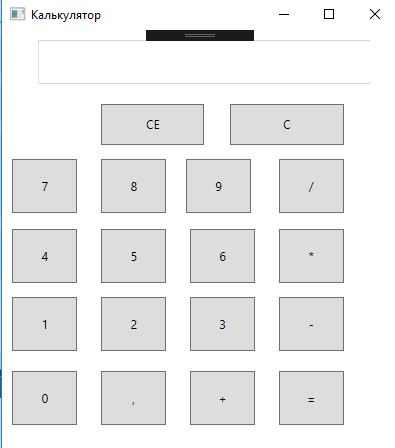
\includegraphics[scale=1]{s1}

	\label{fig:s1}
\end{figure}
Изображен результат работы программы.

Вывод: Создал простейшию программу на языке C\# с использованием WPF. 



